% Gallery figure source
% Summary: Gene trees nested inside a species history. The gray tubes represent species or population branches. Colored lineages represent two loci sampled from species A, B, and C. The blue gene tree coalesces in a way that matches the species tree, while the orange gene tree is discordant because some lineages fail to coalesce until the deeper ancestral population.
\documentclass[tikz,border=6pt]{standalone}
% Shared color palette
\usepackage[T1]{fontenc}
\usepackage[utf8]{inputenc}
\usepackage{lmodern}
\usepackage{microtype}
\usepackage{amsmath,amssymb,mathtools}
\usepackage{xcolor}
\usepackage{tikz}
\usetikzlibrary{arrows.meta,positioning,calc,fit,backgrounds,decorations.pathreplacing,shapes.geometric,shadows.blur}

\definecolor{mainblue}{RGB}{42,85,132}
\definecolor{deepgreen}{RGB}{30,105,70}
\definecolor{burntorange}{RGB}{190,90,25}
\definecolor{softgray}{RGB}{245,246,248}
\definecolor{darkgray}{RGB}{70,70,70}
\definecolor{violet}{RGB}{110,70,150}

\newcommand{\given}{\,|\,}
\newcommand{\Ne}{N_{e}}
\newcommand{\ARG}{\mathrm{ARG}}
\newcommand{\MRCA}{\mathrm{MRCA}}
\newcommand{\GMRCA}{\mathrm{GMRCA}}

% Shared TikZ styles
\tikzset{
  tip/.style={circle,fill=black,inner sep=1.6pt},
  nodept/.style={circle,fill=black,inner sep=1.4pt},
  sampled/.style={rectangle,fill=black,inner sep=2.2pt},
  branch/.style={line width=0.8pt},
  retic/.style={circle,draw=burntorange,fill=burntorange!25,line width=0.8pt,inner sep=2.0pt},
  event/.style={circle,draw=mainblue,fill=mainblue!15,line width=0.8pt,inner sep=1.8pt},
  arr/.style={-{Latex[length=2.0mm]},line width=0.8pt},
  faint/.style={line width=0.7pt,draw=gray!55},
  parentedge/.style={-{Latex[length=2.0mm]},line width=0.9pt,draw=burntorange},
  treeedge/.style={-{Latex[length=2.0mm]},line width=0.9pt,draw=black},
  segment/.style={line width=4pt,line cap=round},
  dashedretic/.style={-{Latex[length=2.0mm]},line width=0.9pt,draw=burntorange,dashed}
}


\begin{document}
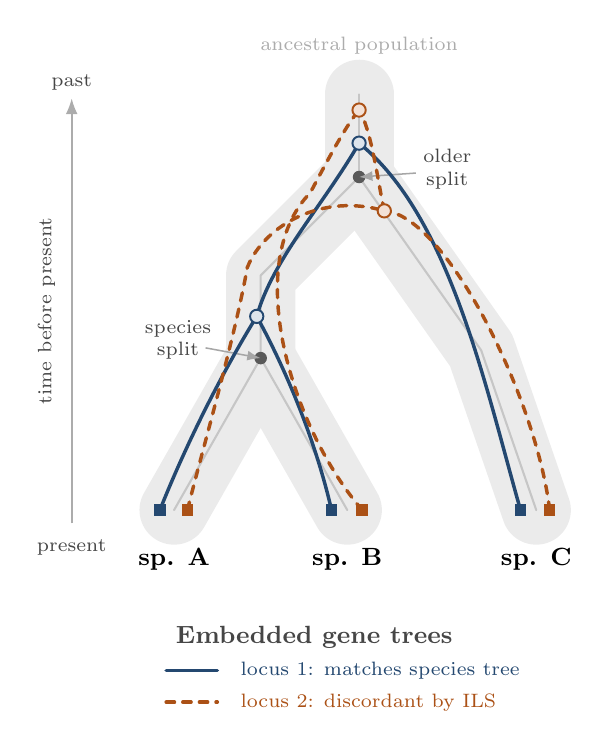
\begin{tikzpicture}[
  scale=1.0,
  tubeback/.style={
    line width=25pt,
    draw=gray!16,
    line cap=round,
    line join=round
  },
  tubeedge/.style={
    line width=.75pt,
    draw=gray!45,
    line cap=round,
    line join=round
  },
  geneone/.style={
    line width=1.25pt,
    draw=mainblue!85!black,
    line cap=round,
    line join=round
  },
  genetwo/.style={
    line width=1.25pt,
    draw=burntorange!90!black,
    dashed,
    line cap=round,
    line join=round
  },
  coalone/.style={
    circle,
    draw=mainblue!85!black,
    fill=mainblue!16,
    line width=.7pt,
    inner sep=1.7pt
  },
  coaltwo/.style={
    circle,
    draw=burntorange!90!black,
    fill=burntorange!18,
    line width=.7pt,
    inner sep=1.7pt
  },
  sampleone/.style={
    rectangle,
    fill=mainblue!85!black,
    inner sep=2.1pt
  },
  sampletwo/.style={
    rectangle,
    fill=burntorange!90!black,
    inner sep=2.1pt
  },
  specnode/.style={
    circle,
    fill=darkgray!90,
    inner sep=1.6pt
  },
  smalllabel/.style={
    font=\scriptsize,
    align=center,
    text=darkgray
  },
  textnote/.style={
    font=\small,
    align=left,
    text width=4.15cm,
    text=darkgray
  },
  callarr/.style={
    -{Latex[length=1.7mm]},
    line width=.55pt,
    draw=gray!70
  }
]

\coordinate (RootTop)   at (3.00,5.90);
\coordinate (RootSplit) at (3.00,4.85);
\coordinate (ABjoin)    at (1.75,3.60);
\coordinate (ABsplit)   at (1.75,2.55);
\coordinate (Aend)      at (0.65,0.62);
\coordinate (Bend)      at (2.85,0.62);
\coordinate (Cmid)      at (4.55,2.65);
\coordinate (Cend)      at (5.25,0.62);

\begin{scope}[on background layer]
  \draw[tubeback] (RootTop)--(RootSplit);
  \draw[tubeback] (RootSplit)--(ABjoin)--(ABsplit);
  \draw[tubeback] (RootSplit)--(Cmid)--(Cend);
  \draw[tubeback] (ABsplit)--(Aend);
  \draw[tubeback] (ABsplit)--(Bend);
\end{scope}

\draw[tubeedge] (RootTop)--(RootSplit);
\draw[tubeedge] (RootSplit)--(ABjoin)--(ABsplit);
\draw[tubeedge] (RootSplit)--(Cmid)--(Cend);
\draw[tubeedge] (ABsplit)--(Aend);
\draw[tubeedge] (ABsplit)--(Bend);

\node[specnode] at (RootSplit) {};
\node[specnode] at (ABsplit) {};

\node[smalllabel,text=gray!65] at (3.00,6.52)
  {ancestral population};

\node[smalllabel] at (0.70,2.78)
  {species\\split};
\draw[callarr] (1.05,2.68)--(ABsplit);

\node[smalllabel] at (4.12,4.95)
  {older\\split};
\draw[callarr] (3.72,4.90)--(RootSplit);

\node[font=\small\bfseries] at (0.65,0) {sp. A};
\node[font=\small\bfseries] at (2.85,0) {sp. B};
\node[font=\small\bfseries] at (5.25,0) {sp. C};

\coordinate (Aone) at (0.47,0.62);
\coordinate (Bone) at (2.65,0.62);
\coordinate (Cone) at (5.05,0.62);

\coordinate (coalAB)   at (1.70,3.08);
\coordinate (coalABC)  at (3.00,5.28);

\draw[geneone]
  (Aone) .. controls (0.80,1.45) and (1.25,2.35) .. (coalAB);

\draw[geneone]
  (Bone) .. controls (2.46,1.45) and (2.10,2.35) .. (coalAB);

\draw[geneone]
  (coalAB) .. controls (1.90,3.80) and (2.55,4.50) .. (coalABC);

\draw[geneone]
  (Cone) .. controls (4.60,2.20) and (4.15,4.35) .. (coalABC);

\node[coalone] at (coalAB) {};
\node[coalone] at (coalABC) {};

\node[sampleone] at (Aone) {};
\node[sampleone] at (Bone) {};
\node[sampleone] at (Cone) {};

\coordinate (Atwo) at (0.82,0.62);
\coordinate (Btwo) at (3.04,0.62);
\coordinate (Ctwo) at (5.42,0.62);

\coordinate (coalAC)  at (3.32,4.42);
\coordinate (coalACB) at (3.0,5.70);

\draw[genetwo]
  (Atwo) .. controls (1.00,1.35) and (1.42,2.80) .. (1.58,3.70)
         .. controls (1.80,4.25) and (2.55,4.65) .. (coalAC);

\draw[genetwo]
  (Ctwo) .. controls (5.26,2.00) and (4.12,4.36) .. (coalAC);

\draw[genetwo]
  (coalAC) .. controls (3.25,4.72) and (3.16,5.45) .. (coalACB);

\draw[genetwo]
  (Btwo) .. controls (2.15,1.65) and (1.50,3.75) .. (2.38,4.65)
         .. controls (2.62,5.10) and (2.83,5.50) .. (coalACB);

\node[coaltwo] at (coalAC) {};
\node[coaltwo] at (coalACB) {};

\node[sampletwo] at (Atwo) {};
\node[sampletwo] at (Btwo) {};
\node[sampletwo] at (Ctwo) {};

\draw[-{Latex[length=2mm]},draw=gray!65,line width=.7pt]
  (-0.65,0.45)--(-0.65,5.85);

\node[smalllabel,rotate=90] at (-0.97,3.15)
  {time before present};
\node[smalllabel] at (-0.65,6.05) {past};
\node[smalllabel] at (-0.65,0.15) {present};

\begin{scope}[xshift=.55cm,yshift=-1cm]
  \node[font=\small\bfseries,text=darkgray,anchor=west] at (0,0)
    {Embedded gene trees};

  \draw[geneone] (0,-0.42)--(0.65,-0.42);
  \node[smalllabel,anchor=west,text=mainblue!85!black] at (0.82,-0.42)
    {locus 1: matches species tree};

  \draw[genetwo] (0,-0.82)--(0.65,-0.82);
  \node[smalllabel,anchor=west,text=burntorange!90!black] at (0.82,-0.82)
    {locus 2: discordant by ILS};
\end{scope}

\end{tikzpicture}
\end{document}
